%!TEX root = ../../dissertation.tex
%%%%%%%%%%%%%%%%%%%%%%%%%%%%%%%%%%%%%%%%%%%%%%%%%%%%%%%%%%%%%%%%%%%%%%%%%%%%%%%
\section{Load Model Queuing Simulation} 
\label{c4:simulation}

As discussed, the solvability of a non-stationary Erlang loss system is very limited. To better tackle this, a simulative approach can be taken. Depending on the level of detail, different types of simulations are available.

Here, a queuing simulation is used to ascertain the blocking probability and tunnel serving slot utilization from the model using the fitted distributions from the trace.


%%%%%%%%%%%%%%%%%%%%%%%%%%%%%%%%%%%%%%%%%%%%%%%%%%%%%%%%%%%%%%%%%%%%%%%%%%%%%%%
\subsection{Queuing Simulation Implementation}

The queuing simulation is implemented on the basis of a \gls{DES}. Instead of reproducing continuous time, this simulation is a series of discrete events. Time is advanced only at these events. 

A queuing model can be easily represented in a \gls{DES}.  Each tunnel request arrival is a modeled as a discrete event. When such an event occurs, three processes are executed. The first process draws a random number from a \gls{PRNG} mapped to \gls{IAT} exponential distribution to schedule the next arrival event. Secondly, the serving units are checked for any free units. If one is found, it will now be occupied. Else, this arrival will be marked as rejected and the third action skipped. This third process now determines the length of the tunnel using another \gls{PRNG} adjusted to the serving time distribution to schedule the event in which the tunnel exits the system.

This model was implemented on the basis of version 3.0 of the \textit{SimPy}~\cite{simpy} package, which is a Python \gls{DES} framework that provides the basic event and scheduling infrastructure. On top of this a base \gls{GGSN} class was constructed, managing the arrival of tunnel events and the scheduling of the service ending events. Specific classes for the traditional (i.e. monolithic) and virtualized (called ``multiserver'' in the code) nodes respectively exist. The implementation is also publicly available\footnote{\url{https://github.com/fmetzger/ggsn-simulation/}} as a reference. 


%%%%%%%%%%%%%%%%%%%%%%%%%%%%%%%%%%%%%%%%%%%%%%%%%%%%%%%%%%%%%%%%%%%%%%%%%%%%%%%
\subsection{Description and Design of the Individual Experiments}

To match the measurement data the simulation time is set to be \SI{7}{\day} in all simulation scenarios. The initial \SI{60}{\minute} of each experiment are considered to be the transient phase and are afterwards deducted from the results. Ten replications of each scenario were performed. All depicted error bars show the \SI{95}{\percent} confidence intervals across the experiments.
%All depicted error bars show the \SI{5}{\percent} and \SI{95}{\percent} quantiles of all replications.

The first experiment was conducted to investigate the normalized baseline load a monolithic \gls{GGSN} experiences using the presented model. Using this, a maximum to the number of concurrent tunnels and the correlation to the blocking probability and tunnel rejection rate can be established. The effects of scaling up, improving the hardware capabilities of the single node, can thus be investigated.

Based on these results, the virtualization and scaling out effects in the virtualized, \gls{GGSN} model are examined. In order to study the feasibility of this approach the performance indicators of the virtual \gls{GGSN} are compared to the baseline established in the first experiment. To this end, the virtual \gls{GGSN} is simulated in configurations varying the number of instances and supported concurrent tunnels per instance.

In a final experiment the startup and shutdown duration of virtual instances and the life cycle management of these instances are additionally taken into account. Although the boot duration of modern \glspl{os} and \glspl{VM}, especially on current hardware with flash storage, is significantly lower than it has been in the past, there is still a delay. This could cause further blocking if the load balancer does not account for this. But the more generously the balancer starts instances in advance the smaller the virtualization efficiency gain, especially the energy consumption, will be become. For this reason, the number of active instance is a relevant performance metric in the virtual \gls{GGSN} model.

The experiment varies the boot delay and implements a very simple load balancer rule as baseline. The rule keeps at least one empty instance running in reserve at all times and deactivates instances, when two running instances are completely unused. As this is very generous, virtualization blocking should only occur in cases of very small instances or very rapid arrivals. Realistic provisioning rules can improve on this quite easily. But even this simplistic approach already serves to demonstrate potential benefits.


%%%%%%%%%%%%%%%%%%%%%%%%%%%%%%%%%%%%%%%%%%%%%%%%%%%%%%%%%%%%%%%%%%%%%%%%%%%%%%%
\subsubsection{GGSN Load, Capacity, and Scaling}

First, with the help of the \glspl{IAT} and duration of tunnels calculated in the dataset evaluation, the monolithic \gls{GGSN} model is studied. While these traces provided information on the frequency of new tunnels and the duration they remain active, no reliable information on the number of required supported concurrent tunnels for a given arrival rate could be deduced. 
This experiment evaluates arbitrary values for the \gls{GGSN} tunnel capacity and determines the resulting blocking probability such that a suitable value can be found. This is a typical task in a dimensioning process.

\begin{figure}[htb]
  \centering
  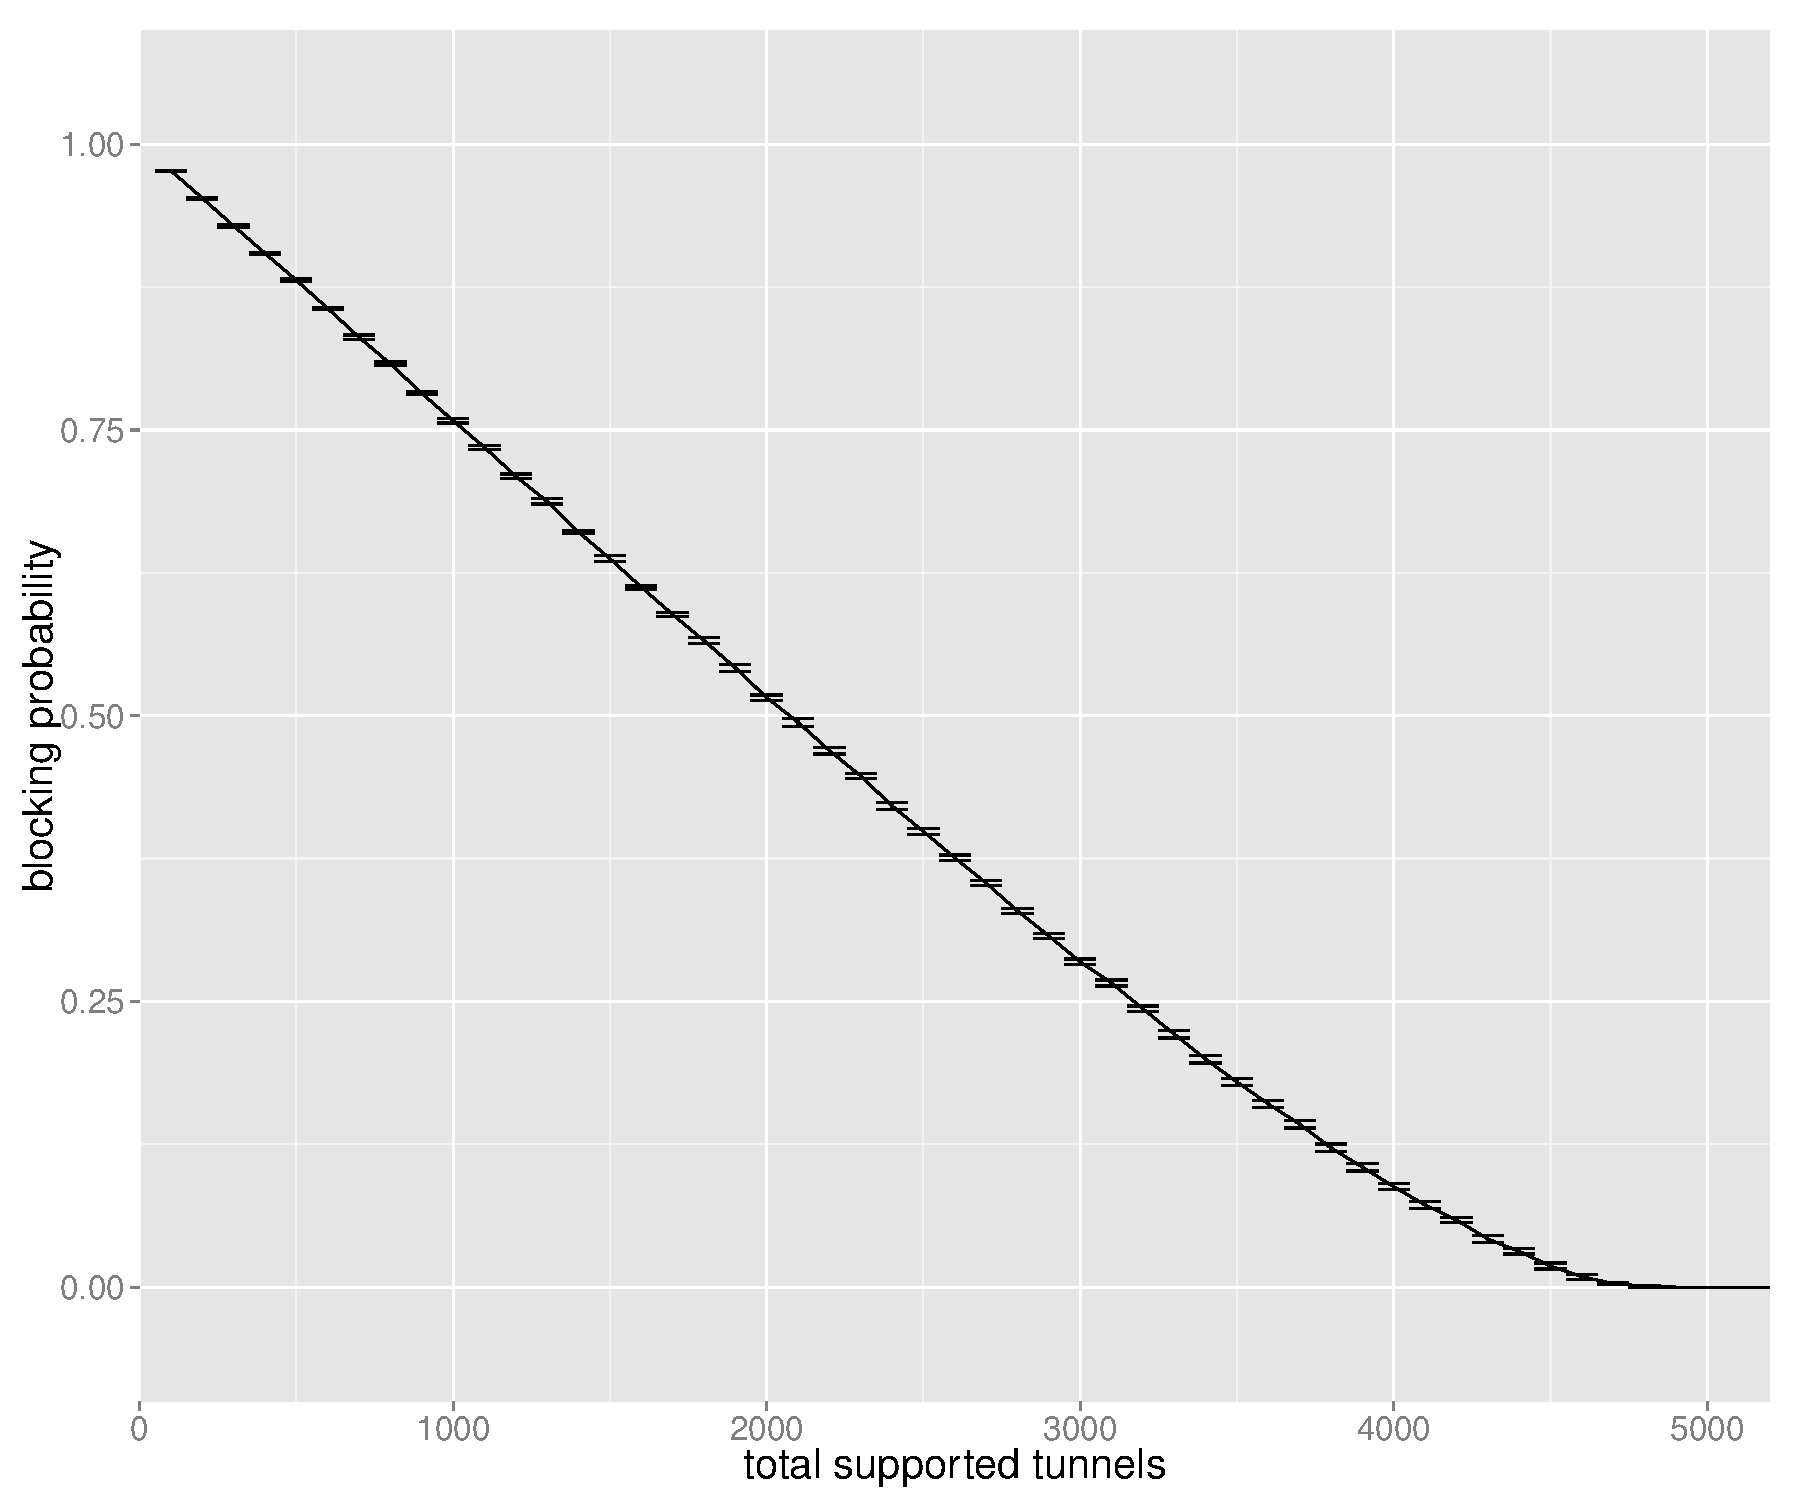
\includegraphics[width=1.0\textwidth]{images/R-monolithic-blocking.pdf}
  \caption{Impact of the number of supported parallel tunnels on the blocking probability for the traditional \gls{GGSN} model. For each scenario the mean and \SI{95}{\percent} confidence intervals of all simulation replications are shown.}
\label{c4:fig:traditional_blocking}
\end{figure}

Figure~\ref{c4:fig:traditional_blocking} studies this impact of the maximum supported number of concurrent tunnels $n$ on the blocking probability $p_B$. $n$ is incrementally increased in steps of \numprint{100} tunnels from \numprint{0} to \numprint{5500}. As expected, the blocking probability decreases with the number of supported tunnels.An almost linear correlation can be observed in the larger part of the graph with a small convergence phase shortly before reaching $p_B=0$. For the normalized inter-arrival no blocking is occurring if a capacity of \numprint{5000} concurrent tunnels is allocated to the \gls{GGSN}.

\begin{figure}[htb]
  \centering
  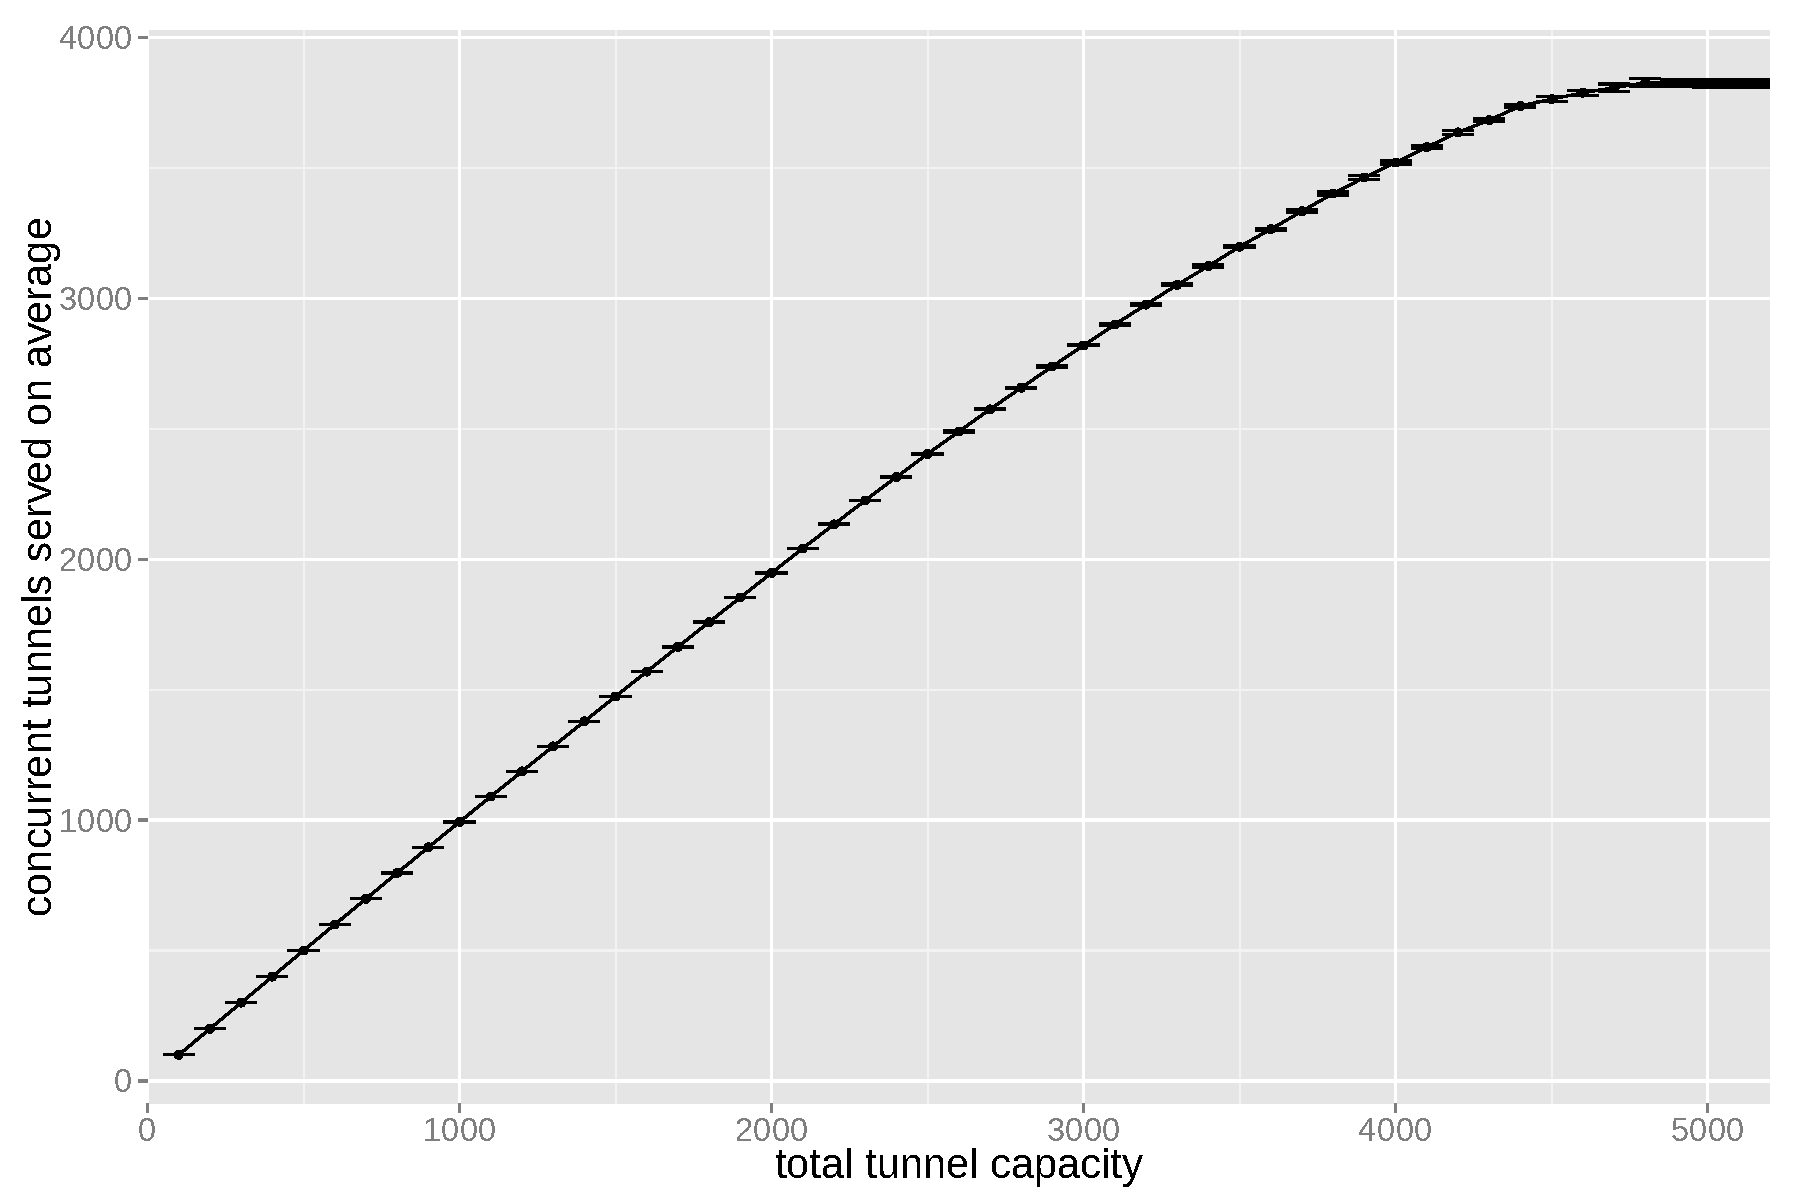
\includegraphics[width=1.0\textwidth]{images/R-monolithic-tunnelusage.pdf}
  \caption{Mean number of tunnels concurrently served by the \gls{GGSN} for incrementally increasing capacity. For each scenario the mean and \SI{95}{\percent} confidence intervals of all simulation replications are shown.}
\label{c4:fig:traditional_tunnelusage}
\end{figure}


A similar picture is also evident in the number of tunnels served by this \gls{GGSN} in the same scenario as shown in Figure~\ref{c4:fig:traditional_tunnelusage}. For the first half of the experiments the \gls{GGSN} is loaded to its limit. Only when the capacity reaches \numprint{4600} can the normalized arrival rate be fully served, which surmounts to about \numprint{3820} tunnels on average in the system. Both results are stable across all simulation runs as the confidence intervals display. For the purpose of network dimensioning the results can be easily scaled up from the normalized arrival rates to the actual ones in the network in question.


%%%%%%%%%%%%%%%%%%%%%%%%%%%%%%%%%%%%%%%%%%%%%%%%%%%%%%%%%%%%%%%%%%%%%%%%%%%%%%%
\subsubsection{Virtualization Impact and Gain}

\begin{figure}[htb]
  \centering
  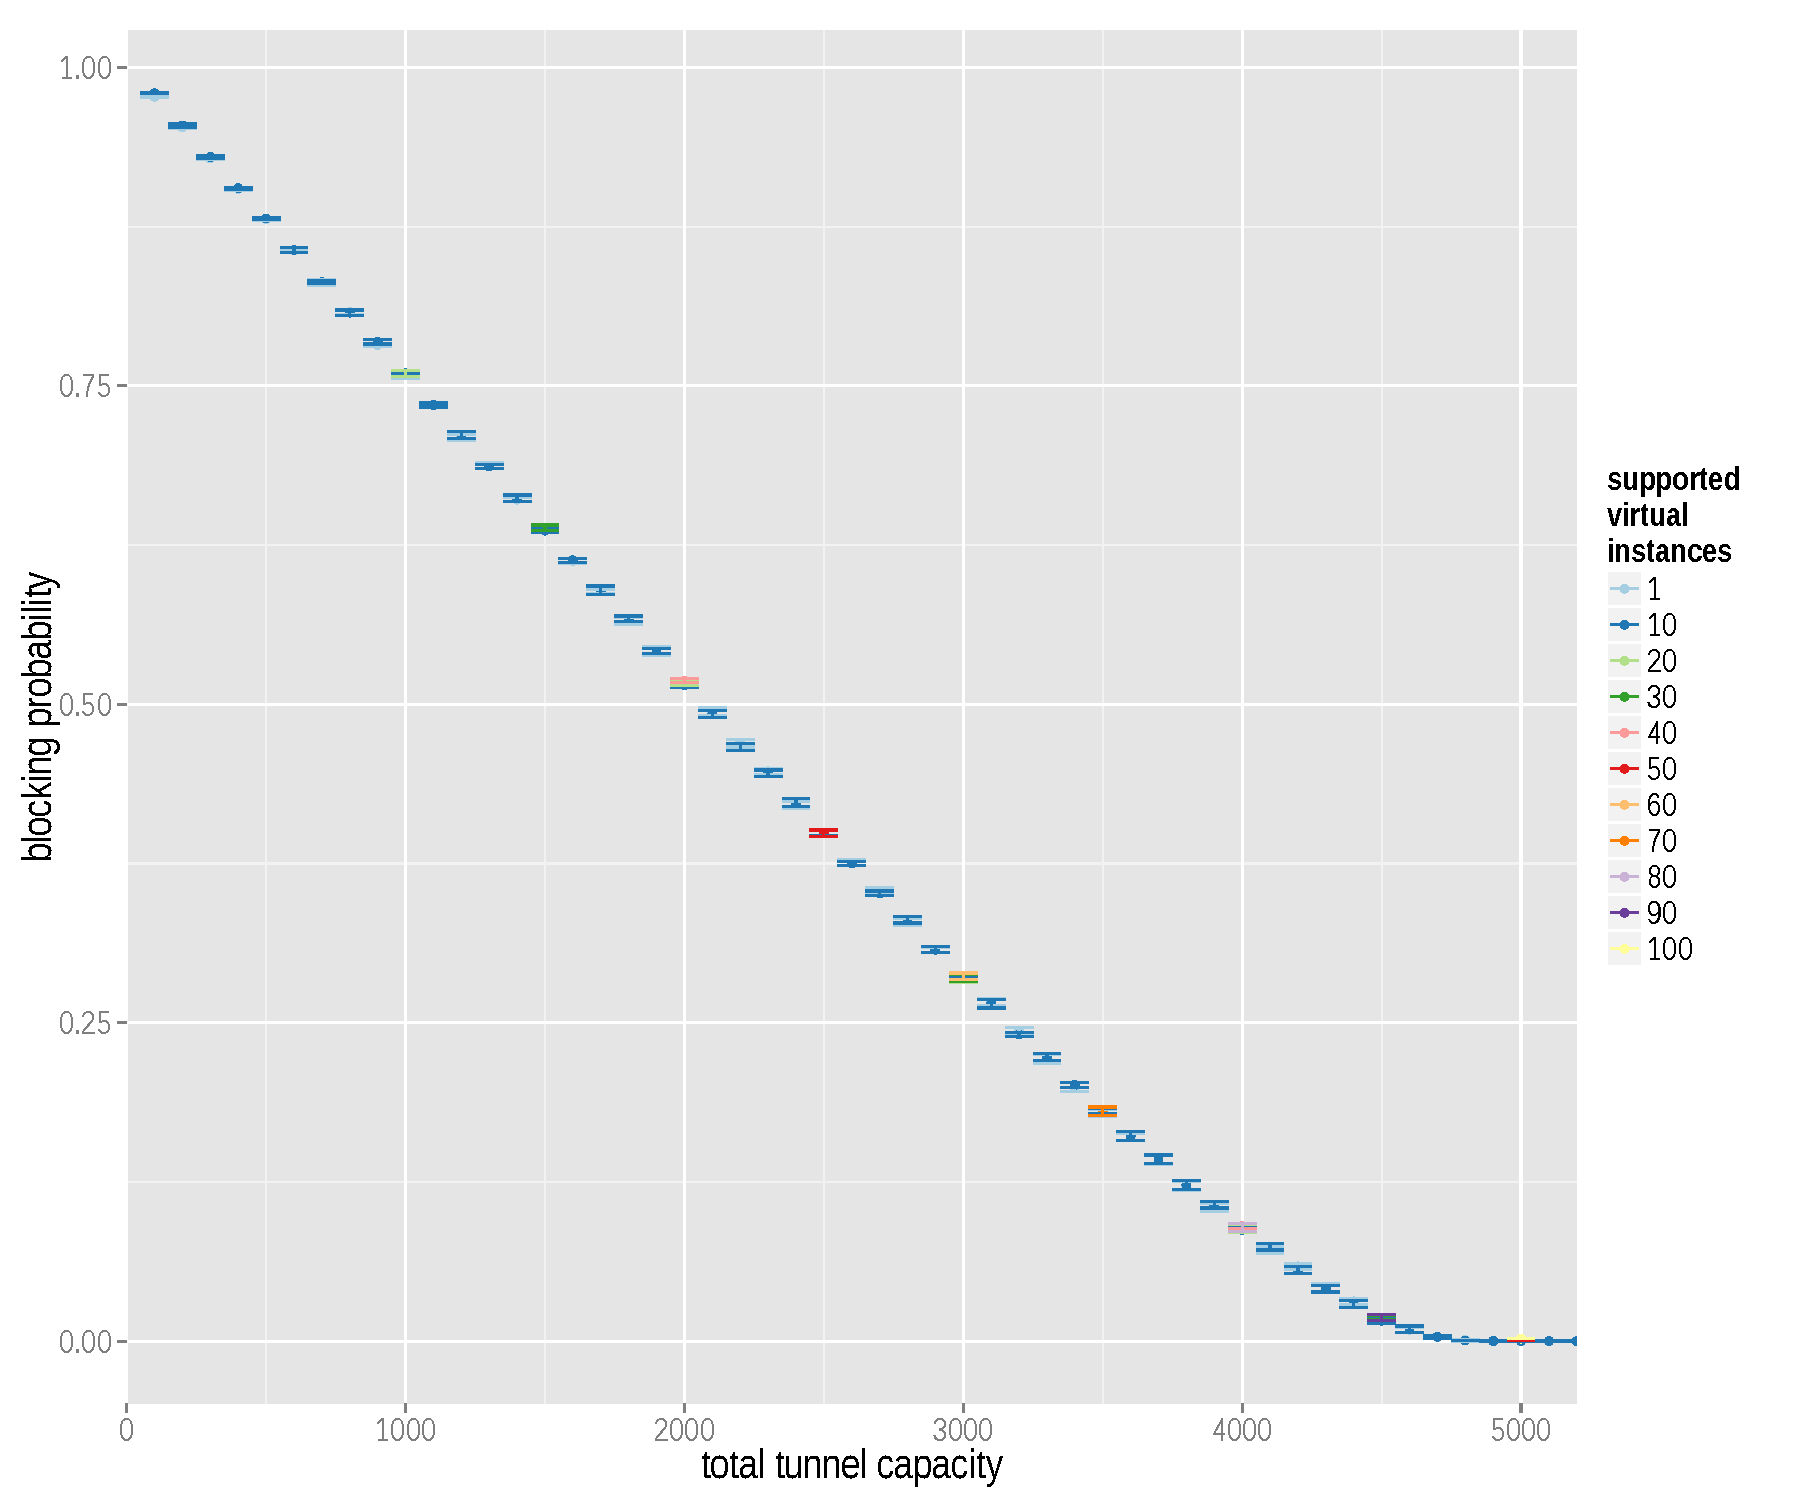
\includegraphics[width=1.0\textwidth]{images/R-virtualized-blocking.pdf}
  \caption{Comparison of the mean blocking probability of various server configurations with \SI{95}{\percent} confidence intervals. The x axis depicts the summary capacity of all virtual instances in the experiment.}
\label{c4:fig:virtualized_blocking}
\end{figure}

\begin{figure}[htb]
  \centering
  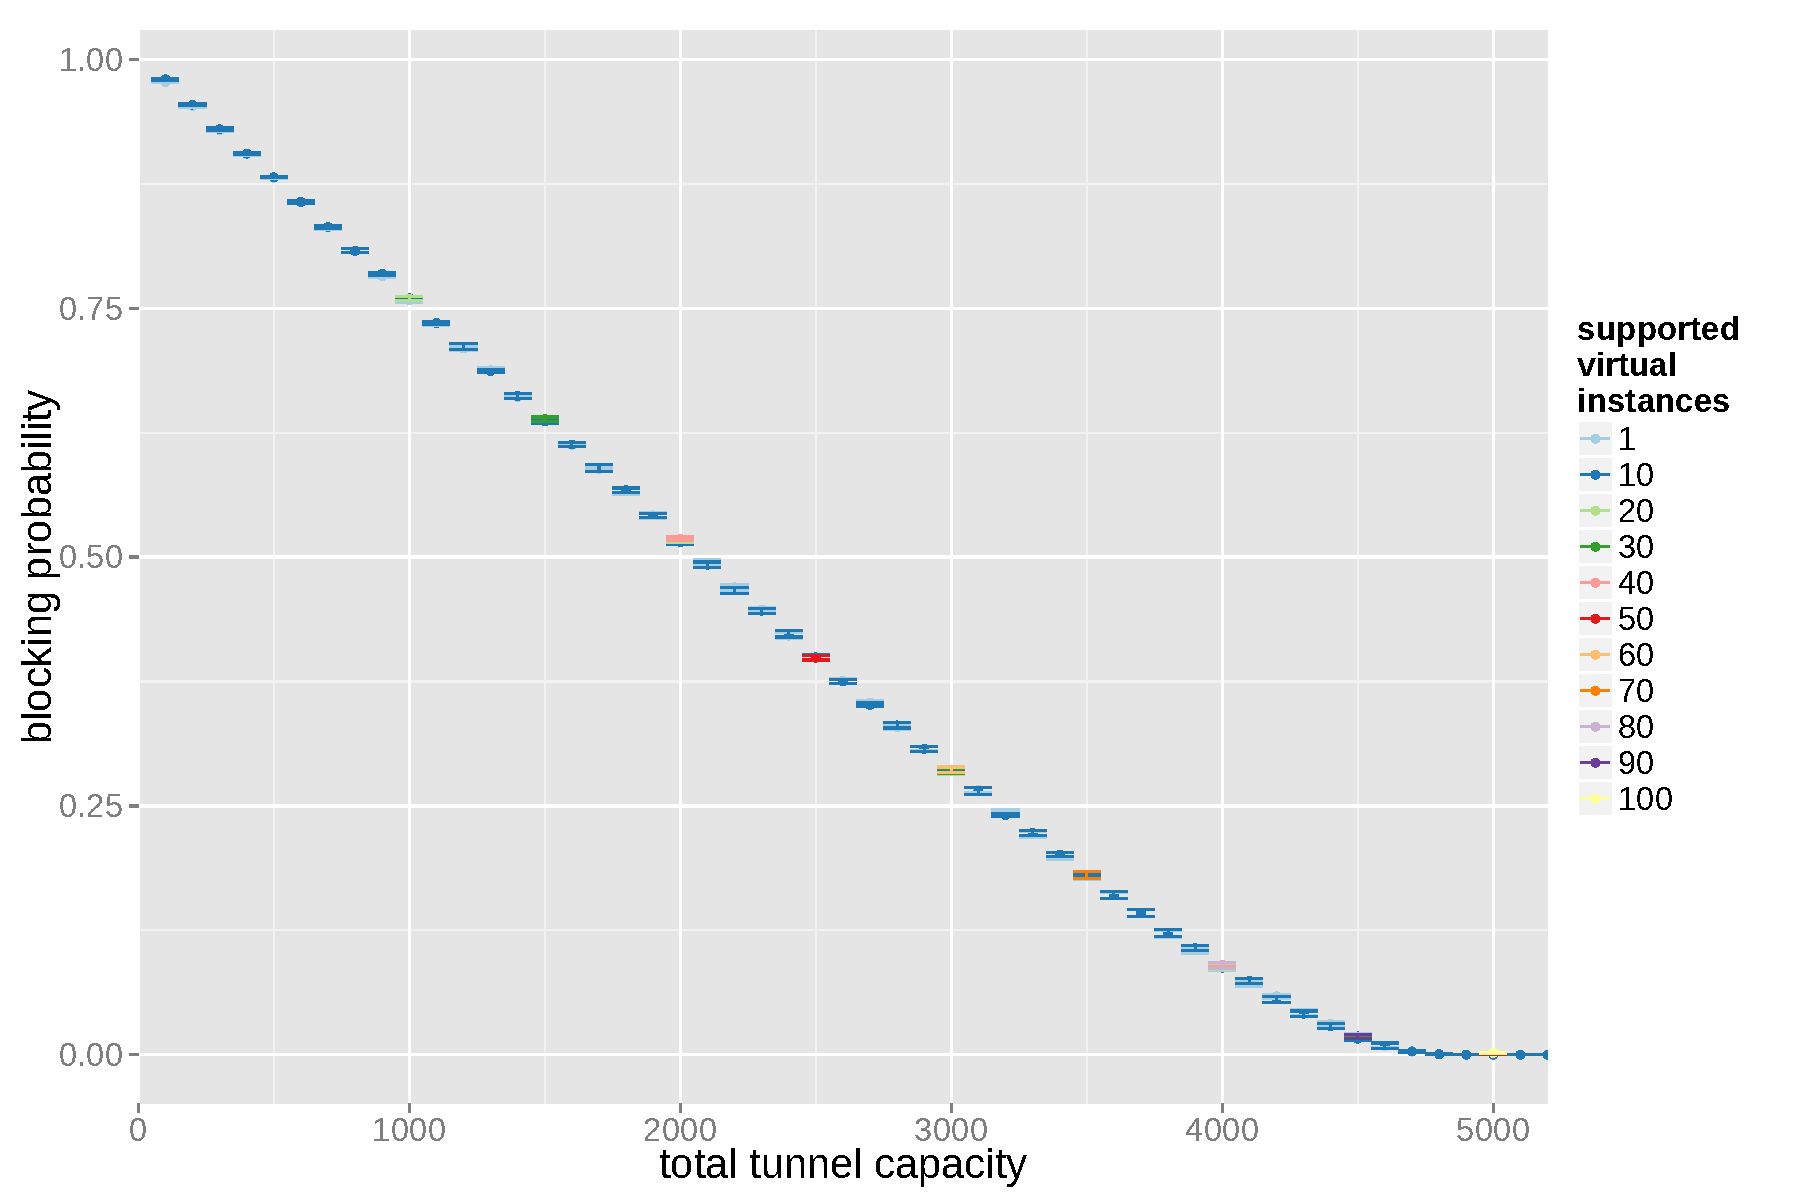
\includegraphics[width=1.0\textwidth]{images/R-virtualized-tunnelusage.pdf}
  \caption{Comparison of the mean tunnel occupation of various virtualization configurations with \SI{95}{\percent} confidence intervals.}
\label{c4:fig:virtualized_tunnelusage}
\end{figure}

A similar experiment can be set up for the virtual \gls{GGSN} model. Learning from the monolithic model, these follow-up simulations can be tuned to the same total tunnel capacity in advance. The only difference is that the tunnel capacity is now spread out evenly between the virtual \gls{GGSN} instances. The experiment tests different amounts for the total number of virtual instances, ranging from \numprint{1}, which represents the monolithic architecture, up to \numprint{100} instances in steps of \numprint{10}.

Figures~\ref{c4:fig:virtualized_blocking} and \ref{c4:fig:virtualized_tunnelusage} demonstrate the results in terms of $p_b$ and concurrent tunnels served overlaid onto the base monolithic scenario's results. No large difference in the results can be seen and the virtualized \gls{GGSN} model behaves no worse than a single large node model.

\begin{figure}[htb]
  \centering
  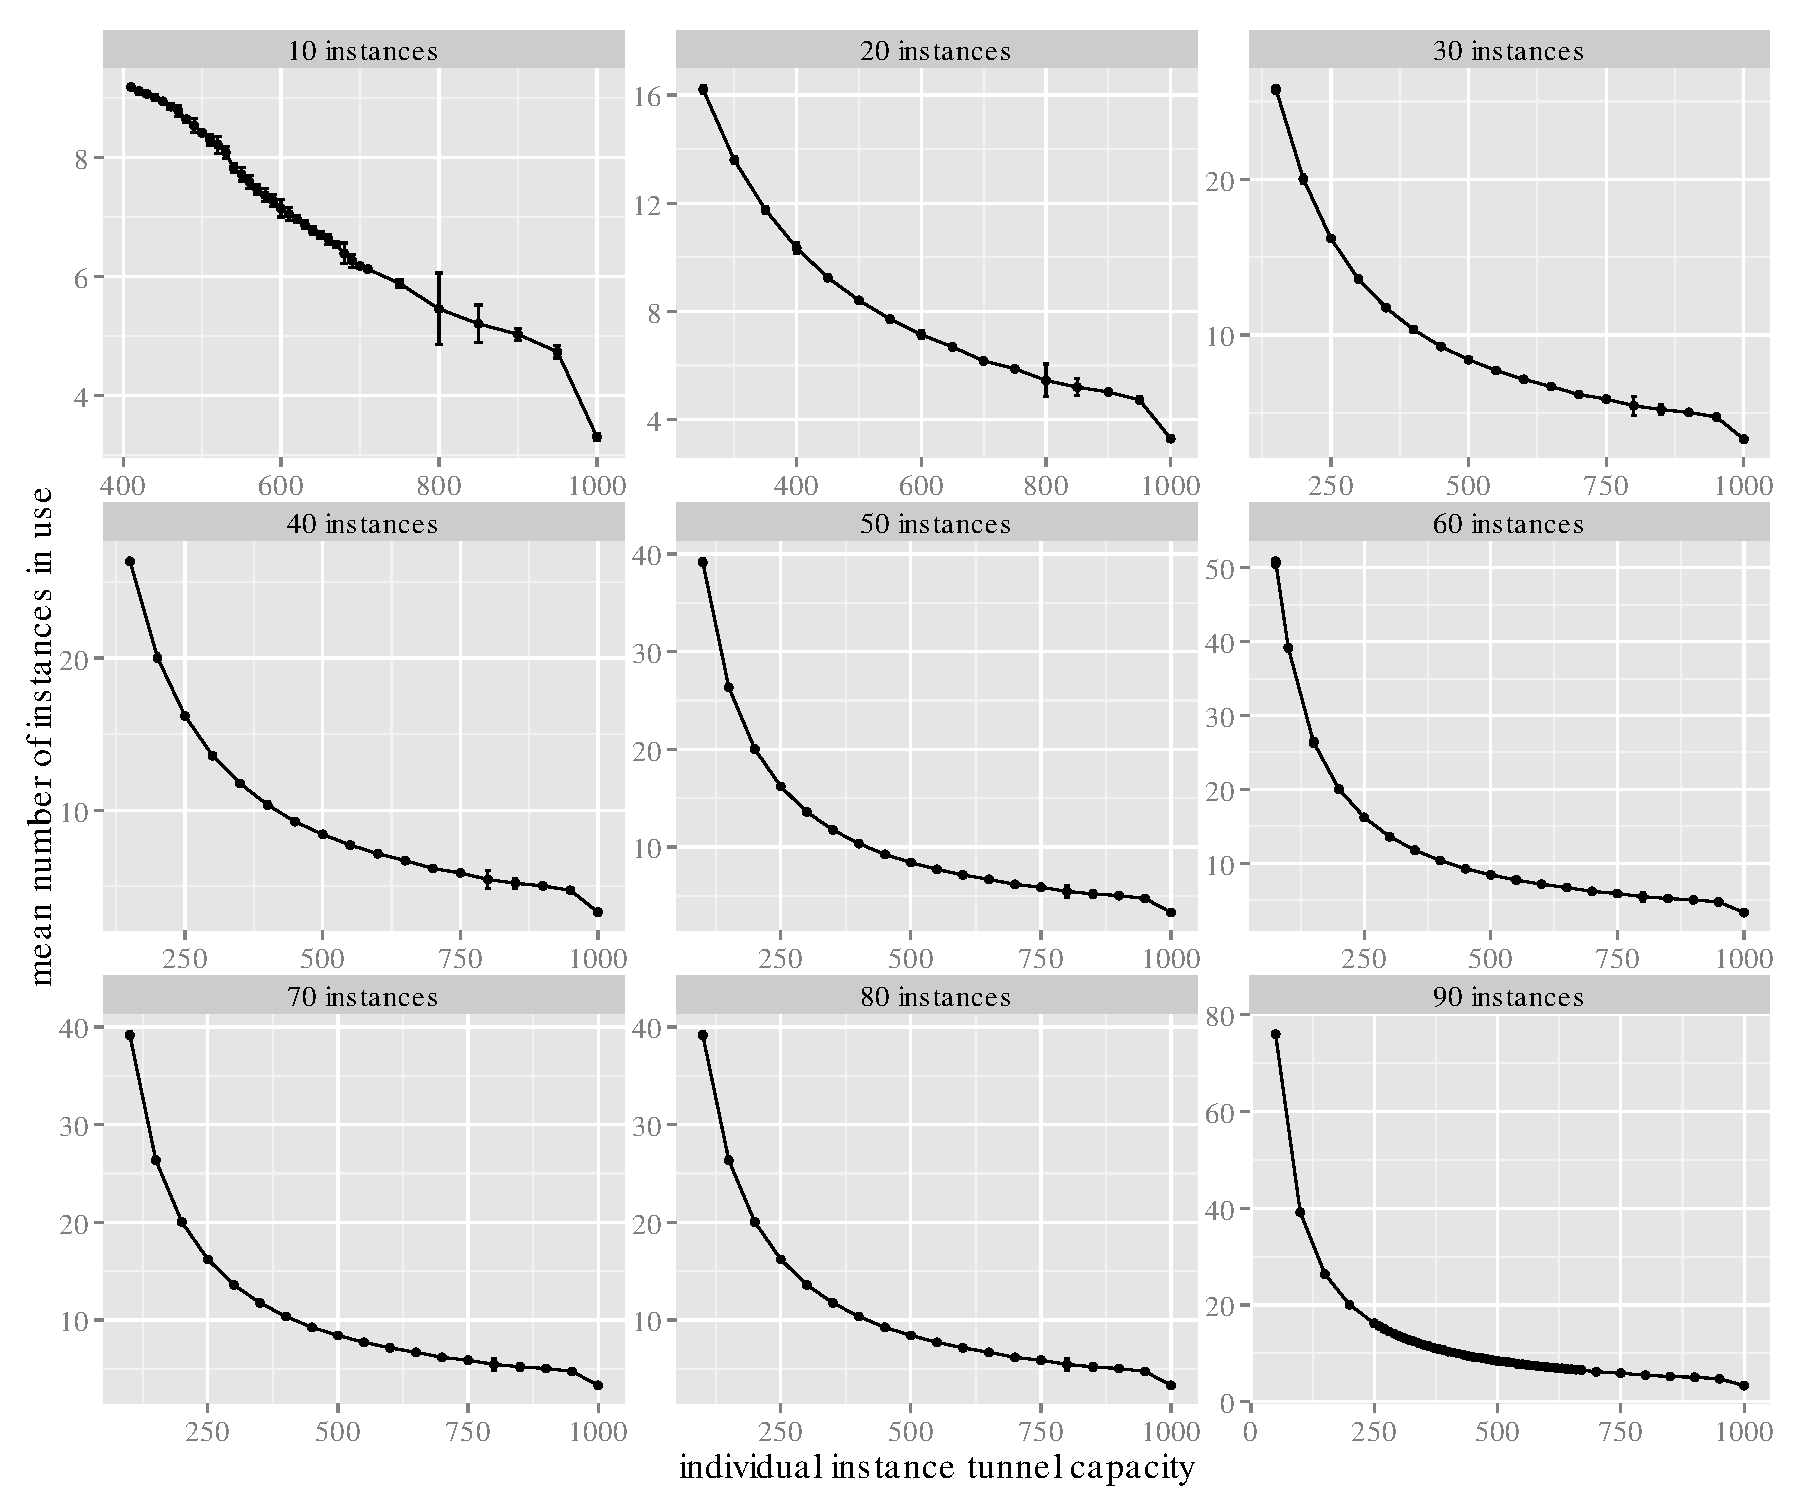
\includegraphics[width=1.0\textwidth]{images/R-virtualized-mean-instanceusage.pdf}
  \caption{Mean instance usage of various virtualization configurations. A higher number of total instances results in a finer granularity of scaling and energy efficiency as more instances can be kept shut down.}
 \label{c4:fig:res-instance-usage-mean}
\end{figure}

But the possible effects of an increased number of instances need to be investigated further. One goal in virtualization is the increase of energy efficiency. This can be achieved by having turned on just as many instances as needed and not more, thus scaling the system to its current load. Therefore, Figure~\ref{c4:fig:res-instance-usage-mean} takes a look at scenarios with nine different instance pools and varying tunnel capacities for each instance. Each setup is compared by the mean number of active instances during the one-week course. The bigger the instances' capacity becomes the less instances need to be active. An actual \gls{GGSN}, even a virtualized one, would need to be dimensioned in such a way to keep the total overhead low. It was already determined that, with the assumed normalized arrival rate, a capacity of \numprint{5000} tunnels is sufficient in order to achieve a blocking probability close to zero. Keeping the setup at this minimum capacity and taking a look at the results in the figure, a good portion of the instances, usually around \SI{20}{\percent}, can still be kept turned off.

\begin{figure}[htb]
  \centering
  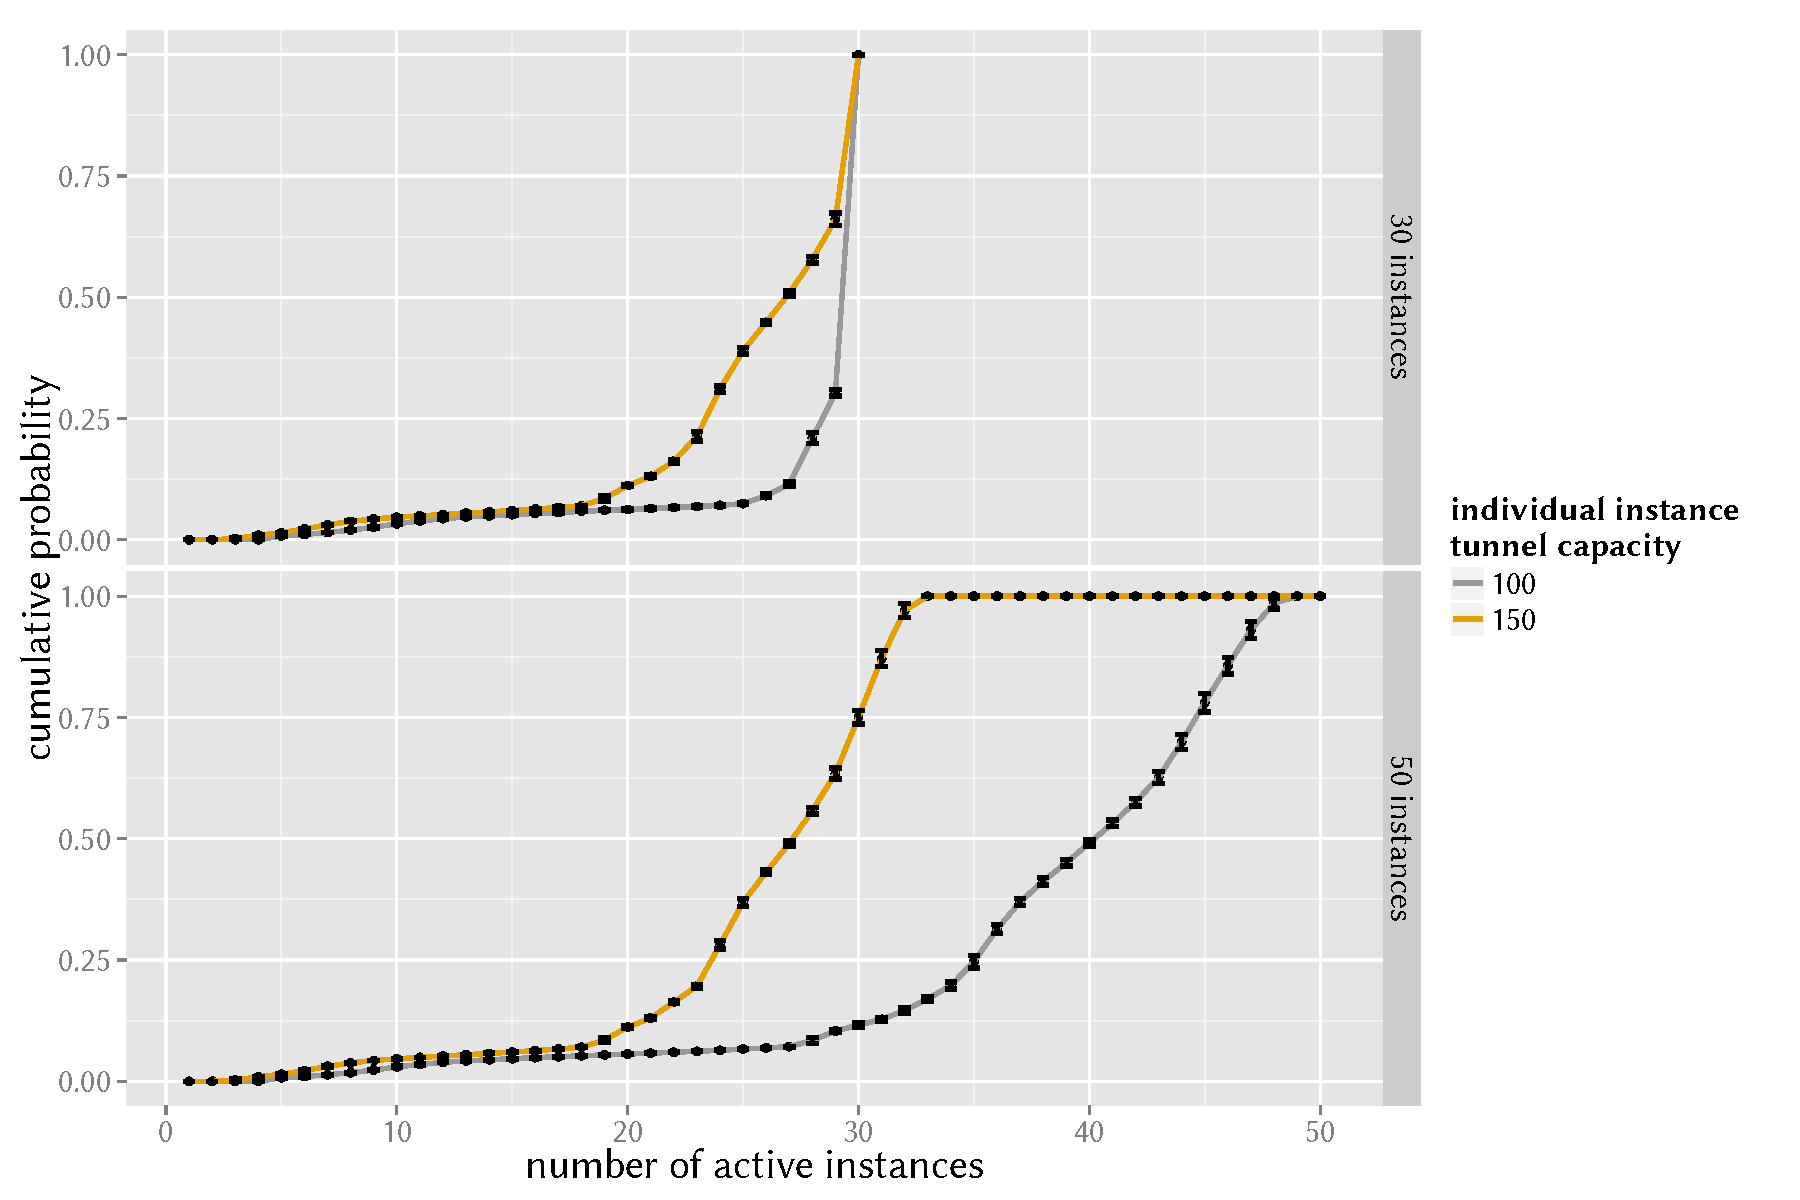
\includegraphics[width=1.0\textwidth]{images/R-virtualized-instanceuse.pdf}
  \caption{Impact of the maximum number of tunnels and number of instances on the number of active instances in the virtual \gls{GGSN} model.}
\label{c4:fig:virtualized_instanceuse}
\end{figure}

To get into more detail, Figure~\ref{c4:fig:virtualized_instanceuse} displays the distribution of the portion of time a specific number of instances was active. Depicted are four configurations differing in their total number of instances and their tunnel capacity. The setup with \numprint{30} instances with \numprint{100} capacity was clearly overwhelmed with the arrival rate and all 30 instances were active over \SI{70}{\percent} of the time. Only when \numprint{150} were allowed the virtualization benefits come into effect and more instances are able to sleep. Similar observations can be made in the \numprint{50} instance case.  Here, the \numprint{100} tunnel scenario is already equipped to handle the tunnel arrival rate and can scale back its active instances quite well, below \numprint{40} instances half the time. The final configuration with a \numprint{150} tunnel capacity is clearly overdimensioned here with no more than \numprint{33} of th \numprint{50} instances ever being active.

\begin{figure}[htb]
  \centering
  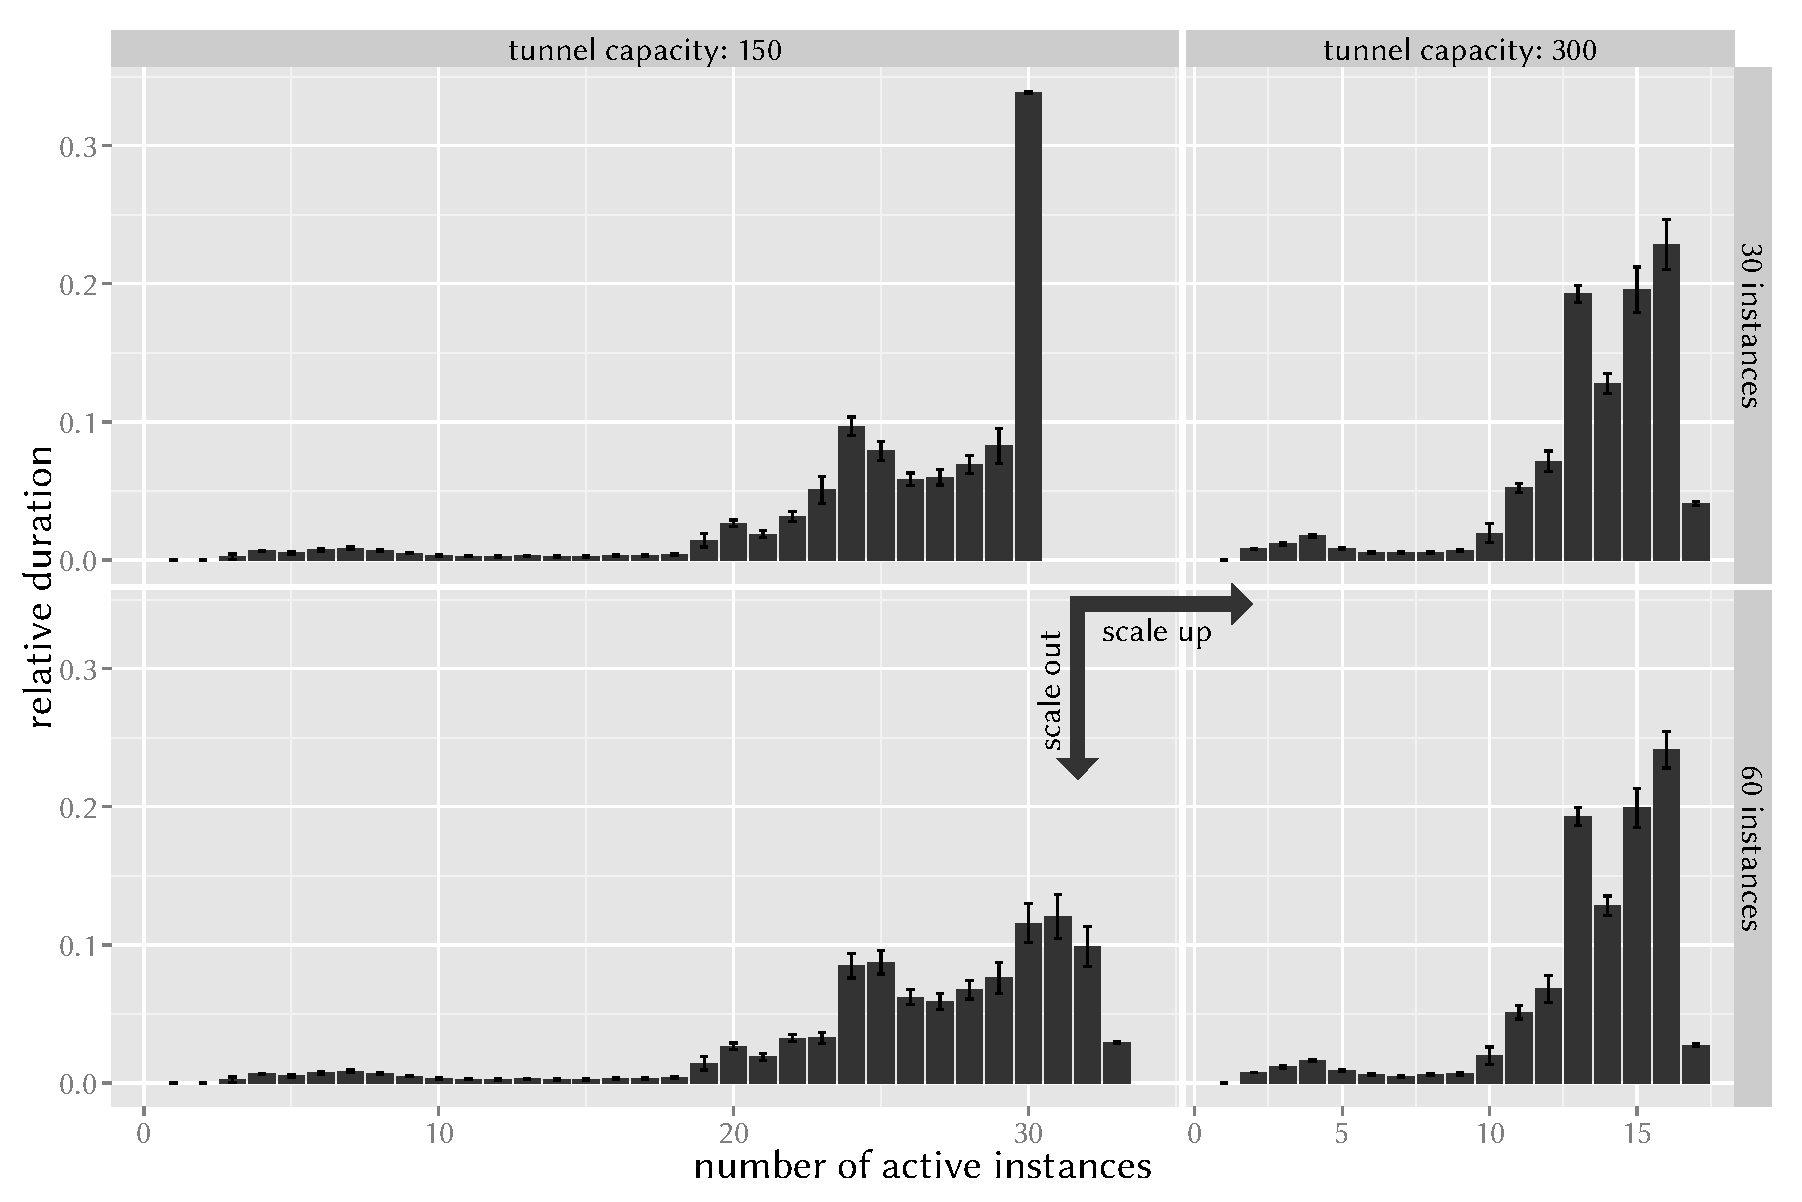
\includegraphics[width=1.0\textwidth]{images/R-virtualized-instanceuse-barplot.pdf}
  \caption{Resource usage from a select maximum virtual instances and tunnel capacity combination, displaying the capability to scale up and out.}
\label{c4:fig:res-usage-barplot}
\end{figure}

Looking at these scenarios and additionally Figure~\ref{c4:fig:res-usage-barplot} from a network dimensioning perspective, one discovers two distinct pathways to scale in the virtualized \gls{GGSN} model. To reach the desired tunnel capacity either the number of instances or the instance's tunnel capacity can be increased. The latter represents the classical scaling up. But virtualization also opens up the new path of scaling out by increasing the number of instances. Through this, scaling can be become easier and cheaper, as existing machines need not be replaced.



%%%%%%%%%%%%%%%%%%%%%%%%%%%%%%%%%%%%%%%%%%%%%%%%%%%%%%%%%%%%%%%%%%%%%%%%%%%%%%%
\subsubsection{Virtual Instance Life Cycle Management Impact}

In this section, we first consider the impact of different boot and shut down times on resource utilization and blocking probabilities. We observe the impact of different start up and shut down times on both resource utilization and blocking probability. Afterwards, the influence of varying server start and stop times on a fixed combination of maximum tunnels and servers in the system is examined.



\begin{figure}[htb]
  \centering
  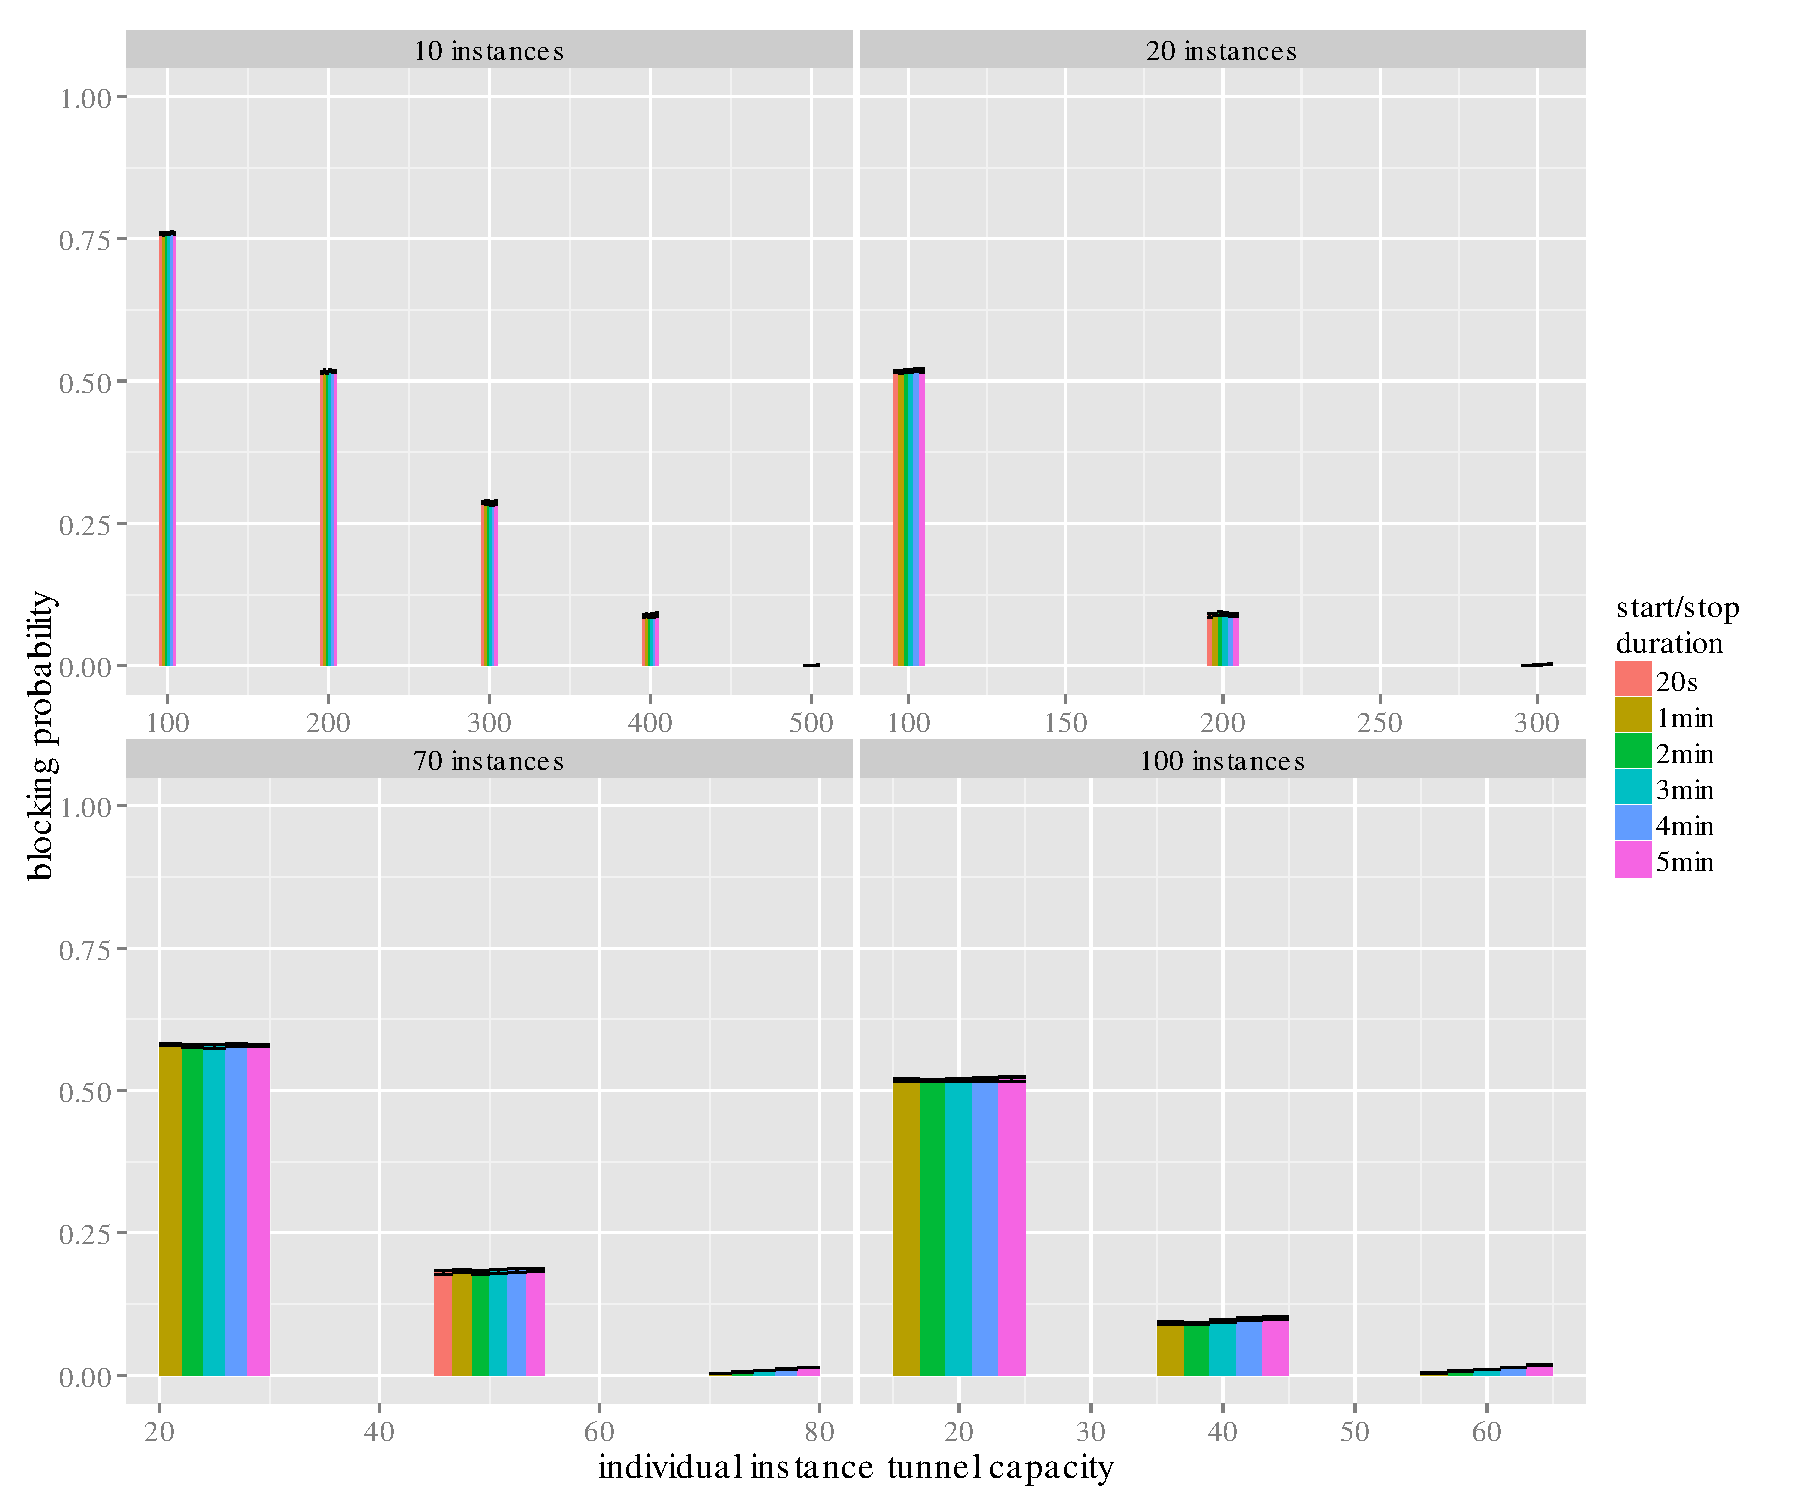
\includegraphics[width=1.0\textwidth]{images/R-virtualized-startstop-blocking-barchart.pdf}
  \caption{Influence of the boot and shutdown time on the blocking probability.}
\label{c4:fig:blockprob-startstop-barchart}
\end{figure}


\begin{figure}[htb]
  \centering
  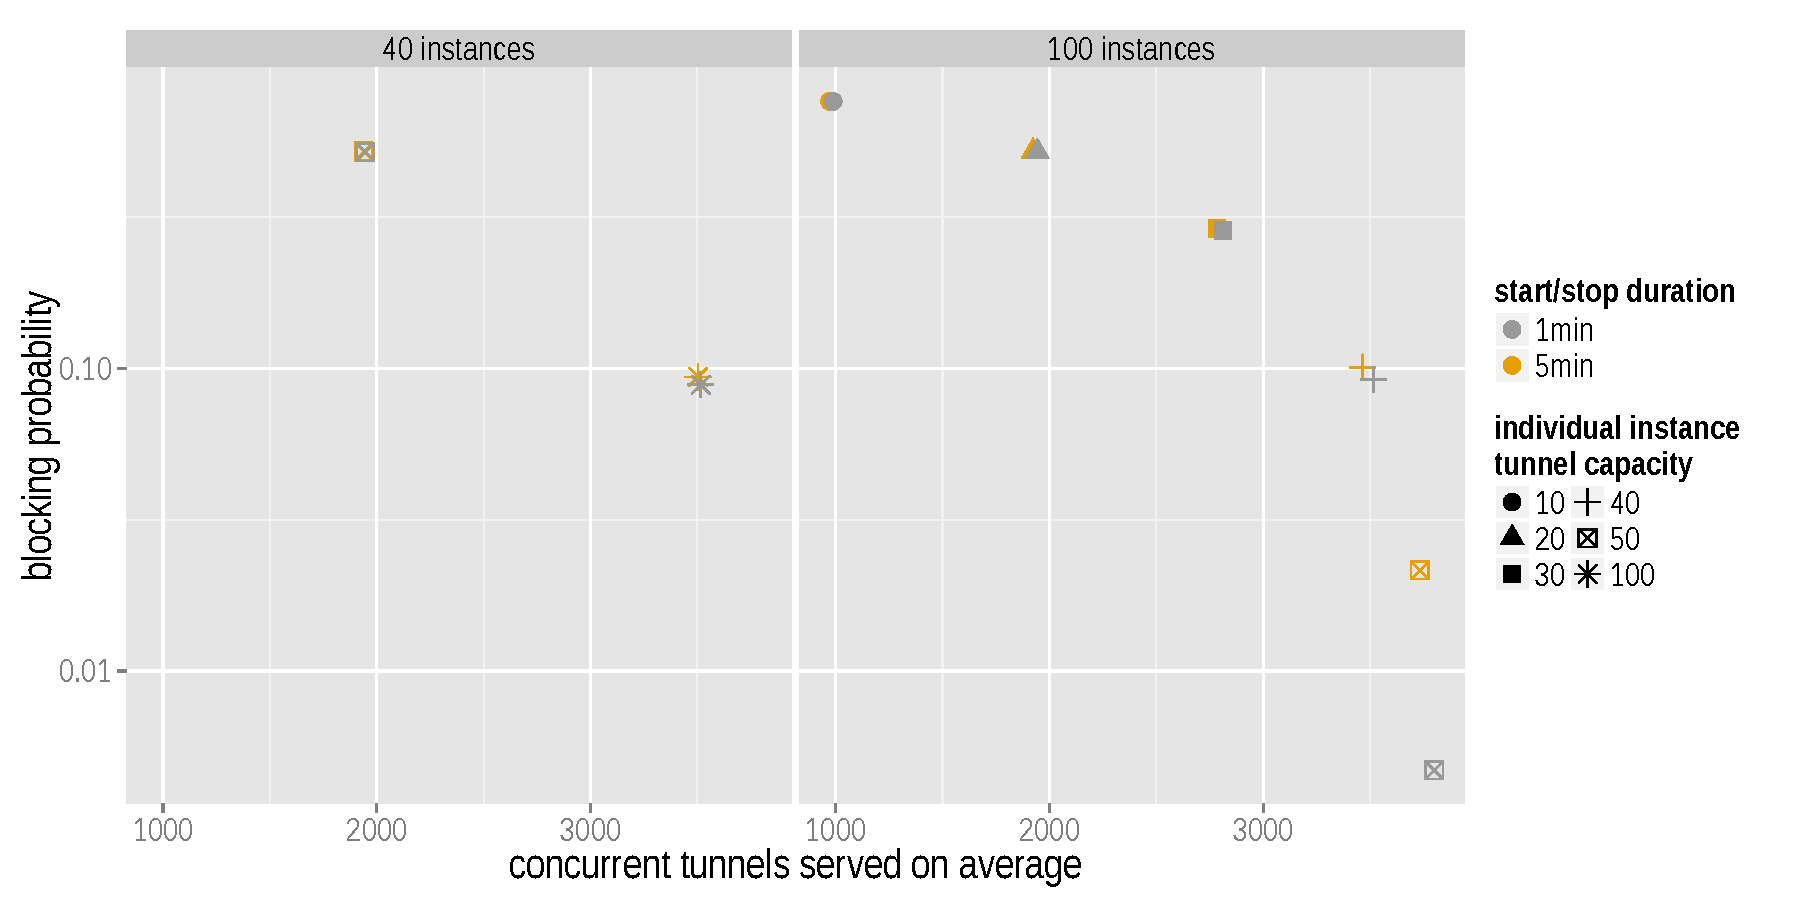
\includegraphics[width=1.0\textwidth]{images/R-virtualized-startstop-tunnelusage-blocking-comparison.pdf}
  \caption{Trade-off between blocking probability and mean resource utilization with regard to maximum number of servers, maximum number of tunnels per server, and start up and shut down time.}
\label{c4:fig:compare_util_block}
\end{figure}



Figure~\ref{c4:fig:compare_util_block} shows scenarios with $40$ and $100$ number of virtual \gls{GGSN} instances and  $1000$ to $5000$ total concurrent tunnels. For each scenario, we study the impact of selecting different maximum numbers of tunnel per server as well as start up and shut down times on blocking probability and mean resource utilization. The first observation is that by increasing the number of servers, i.e. scaling out, the blocking probability can be decreased, while maintaining a relatively low mean resource utilization. In addition to the previous effects, we notice that a higher start up and shut down time causes a slight increase in blocking probability for servers with low tunnel capacity.

\begin{figure}[htb]
  \centering
  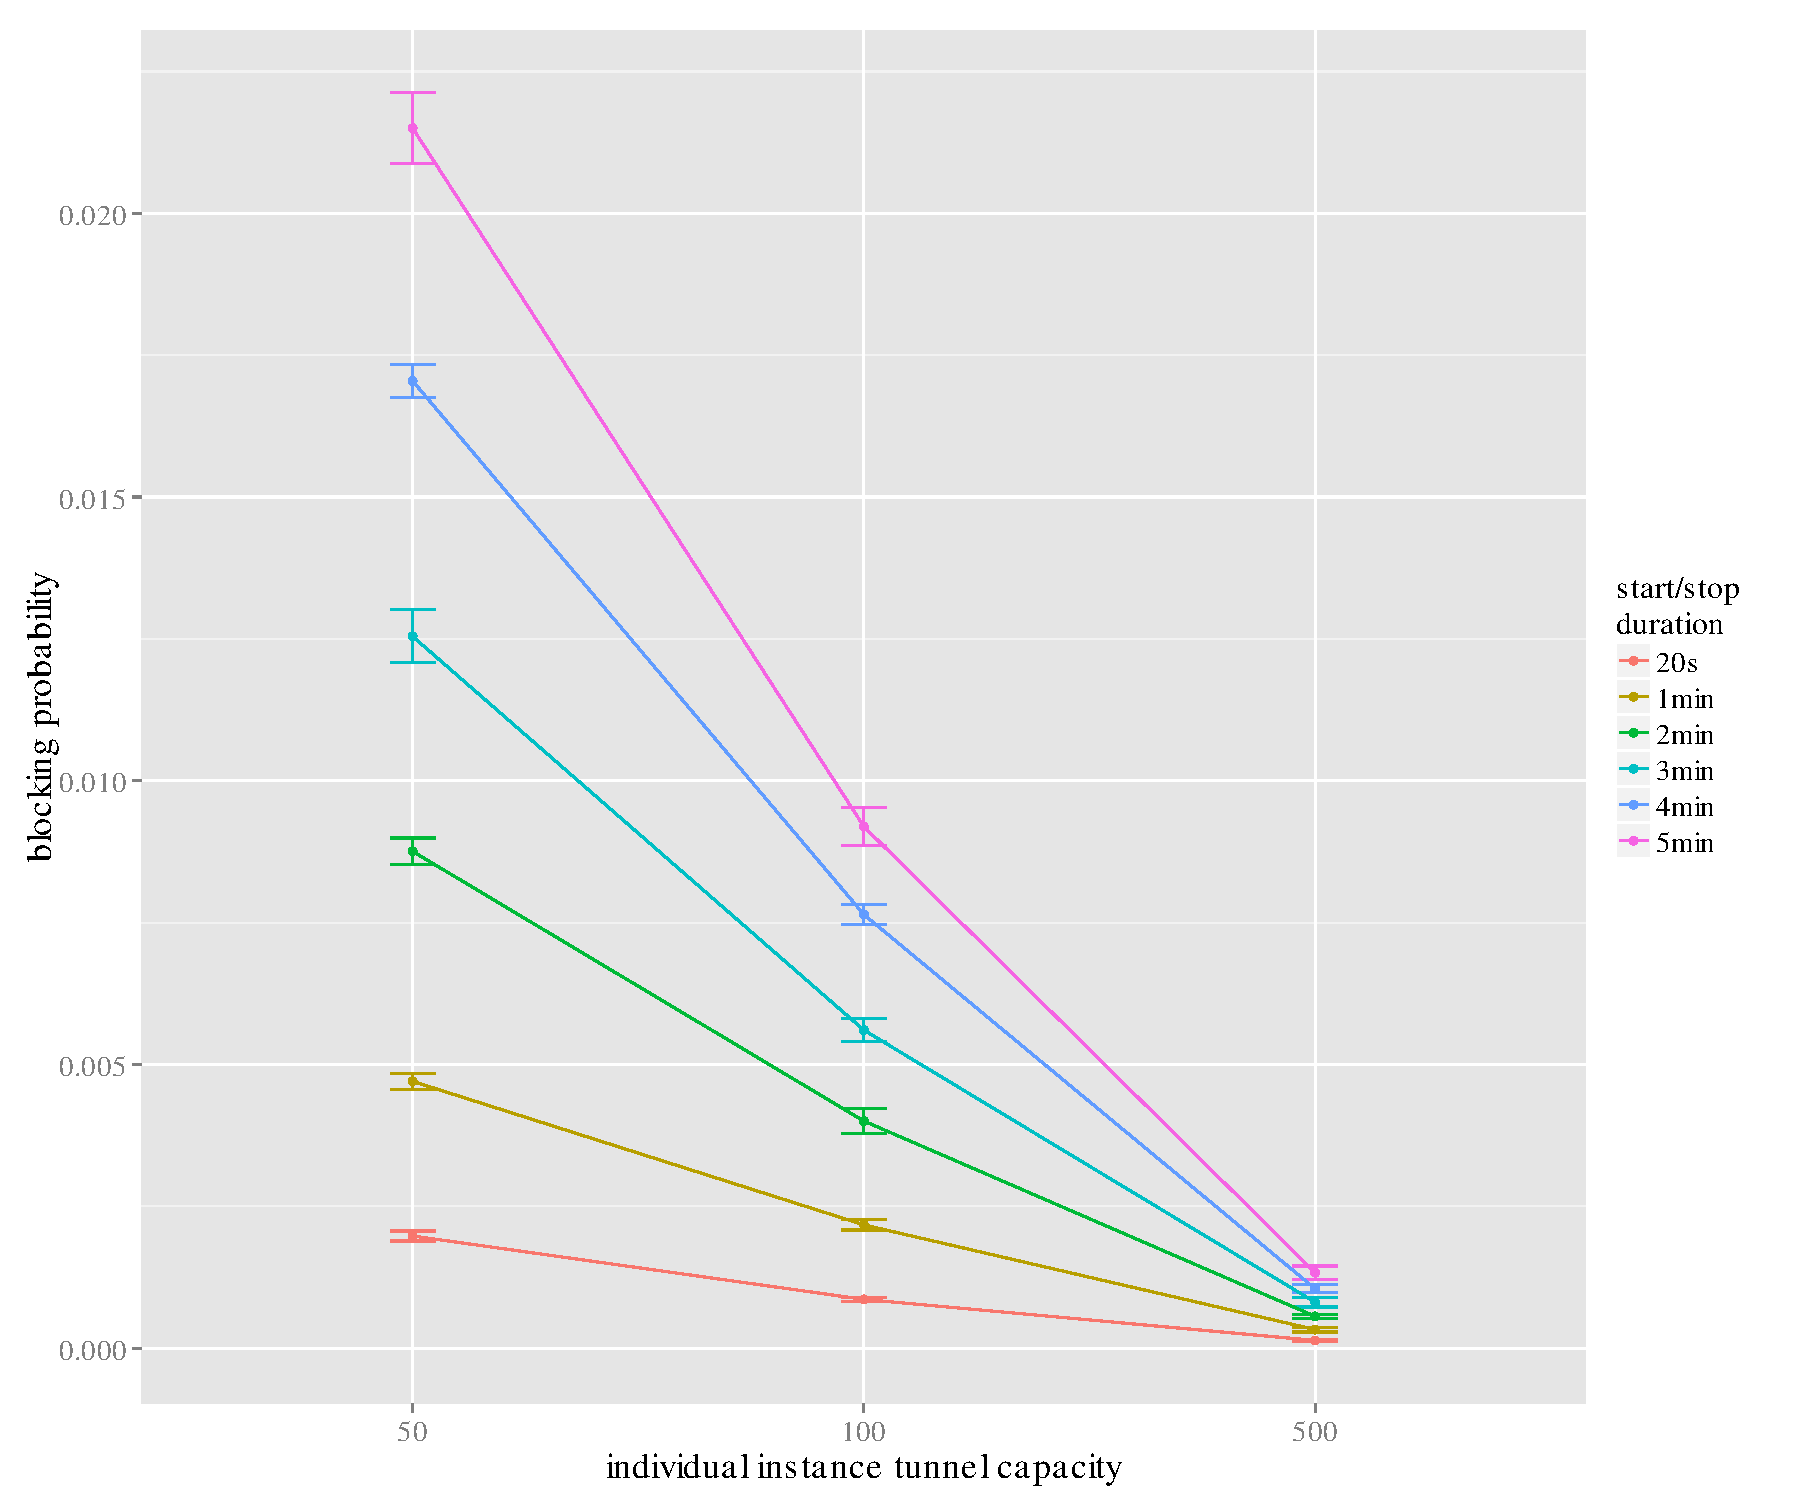
\includegraphics[width=1.0\textwidth]{images/compare-maxinstances-block.pdf}
  \caption{Influence of start up and shut down time on blocking probability with regard to different numbers of servers.}
\label{c4:fig:compare_maxinstances_block}
\end{figure}


In order to study this behavior in more detail, we focus on a specific scenario in Figure~\ref{c4:fig:compare_maxinstances_block}, where $5000$ total tunnels should be supported by the system. In order to achieve this goal, we consider three types of instances, with the server capacity varying between $50$ and $500$.  In each case we change the start up and shut down time between $1$ and $5$ minutes. It can be easily observed, that lower server capacities combined with higher start up and shut down times increase the blocking probability. This is due to the server start up threshold mechanism, used in the model, not taking the additional capacity gained by activating an additional server into account. If a low capacity server with a long boot time is activated, there is a high probability that the system will quickly expend its capacity again.


\begin{figure}[htb]
  \centering
  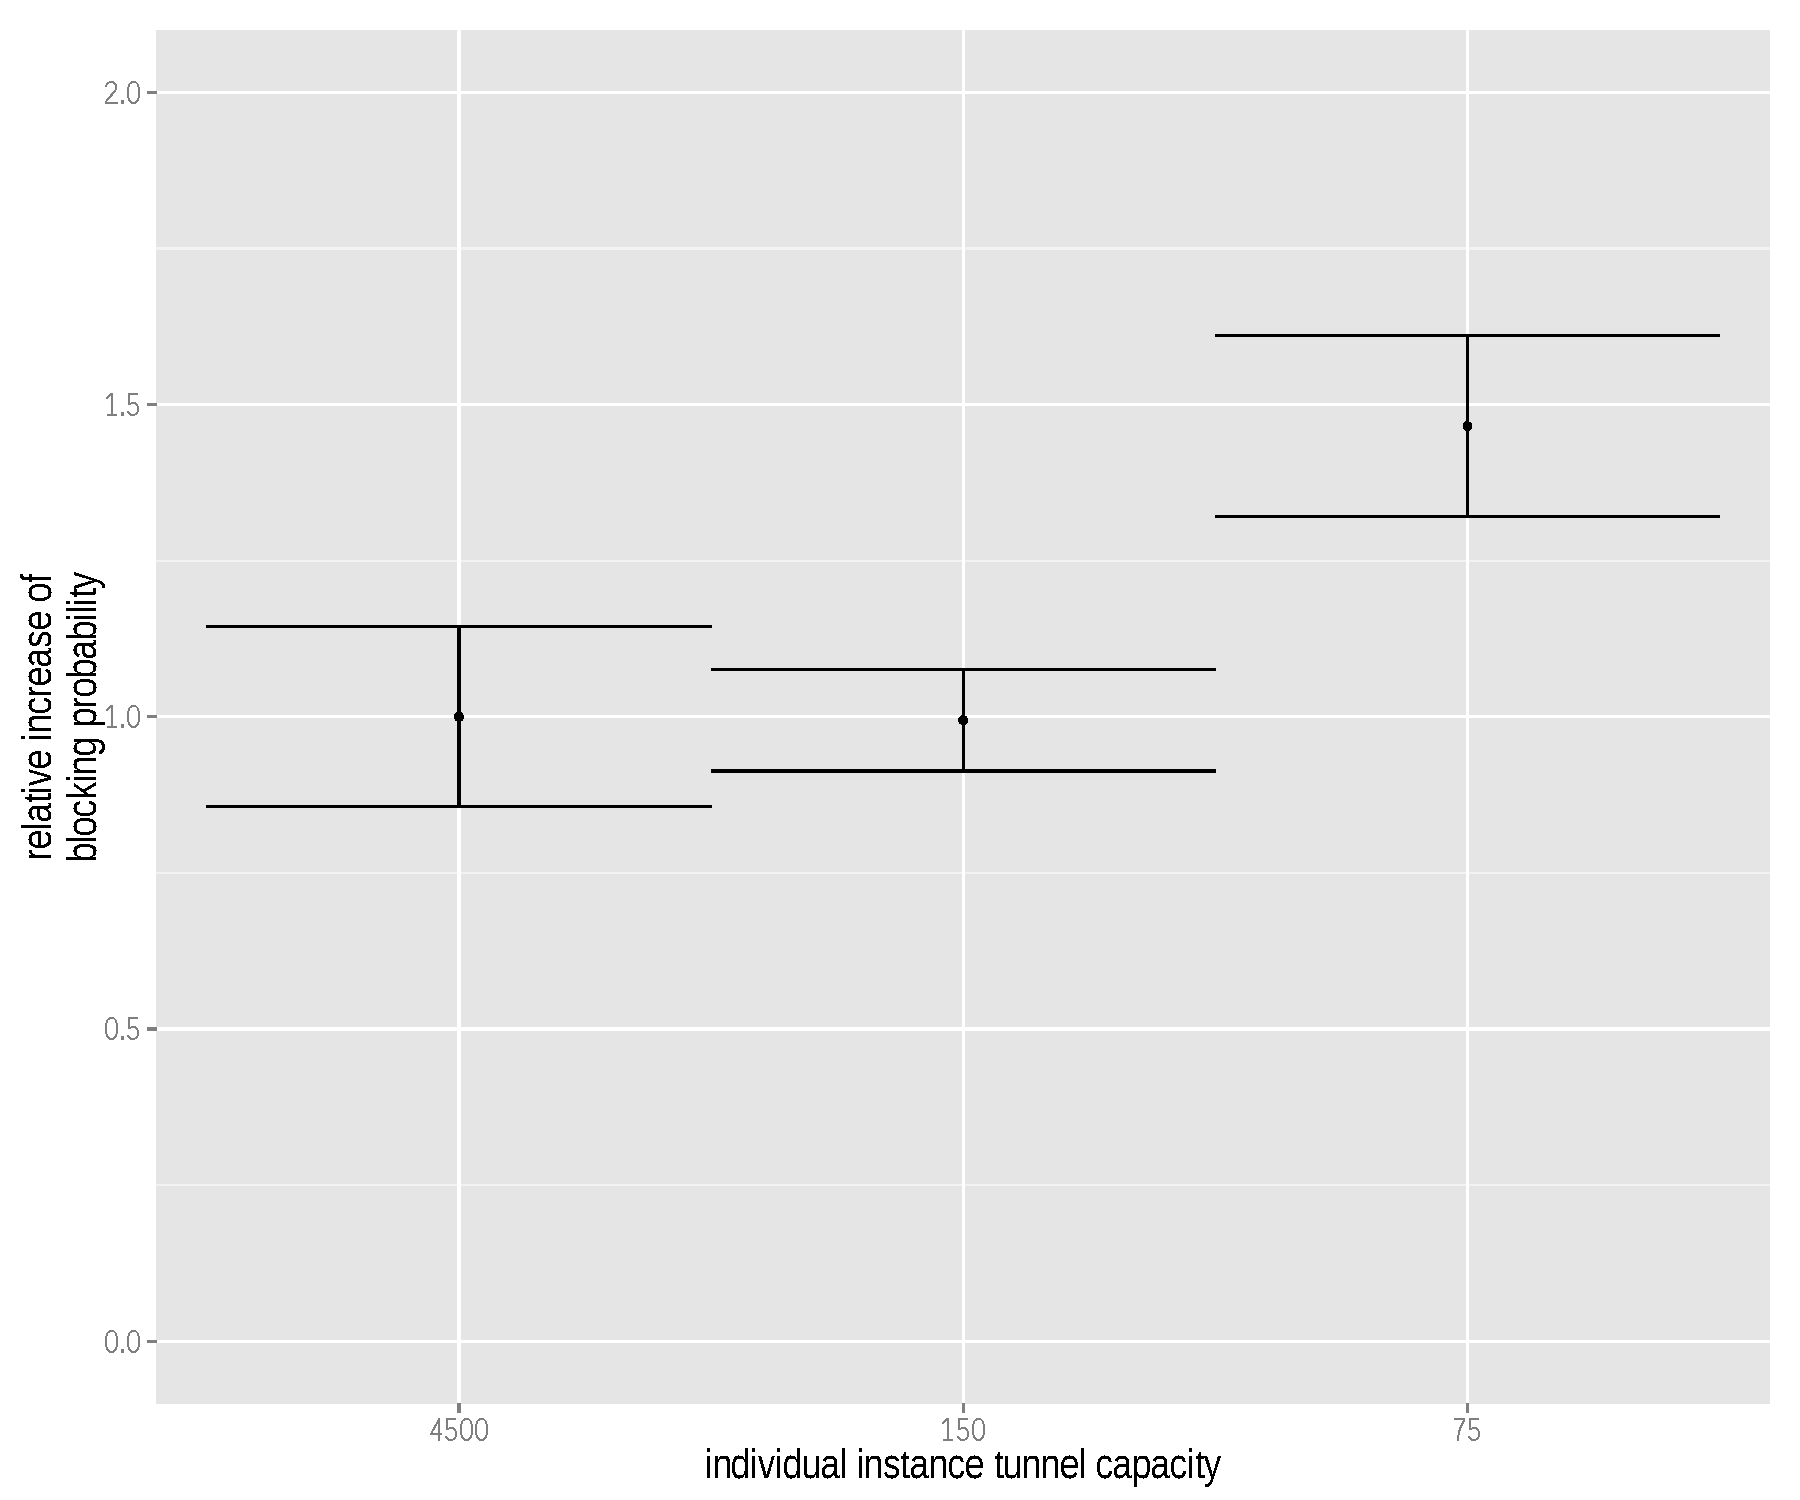
\includegraphics[width=1.0\textwidth]{images/blocking-comparison.pdf}
  \caption{Relative increase of blocking probability on the number of servers compared to the traditional \gls{GGSN}; with the $4500$ maximum tunnels per server being on a single server, $150$ on $30$, and $75$ on $60$ servers.}
\label{c4:fig:blocking-comparison}
\end{figure}

Finally, Figure~\ref{c4:fig:blocking-comparison} takes one last closer look at a potential increase of the blocking probability in virtualized scenarios when compared to the monolithic basis. In theory, virtualization can incur additional overhead which would represent itself as an increase in $p_b$. In our model the overhead can only stem from the hypervisor and its simplistic scheduling  and lifecycle management strategies in conjunction with the instances' boot delay. The figure plots the blocking probability of the traditional \gls{GGSN} system dimensioned for $4500$ concurrent tunnels with the virtual \gls{GGSN}.

We observe that, with the start up and shut down time of $5$ minutes in mind, the blocking probability increases by a factor of $1.48$ if the capacity of each server is set to $75$, i.e. $\frac{1}{60}$ of the original server capacity, while $27$ of all $60$ servers can be turned of or used for other purposes at \SI{50}{\percent} of the time. We conclude, that choosing more powerful servers decreases the blocking probability but reduces the potential to disable servers.

So far we have considered a conservative start up and shut down time of servers of \SI{5}{\minute}, which can potentially occur if current generation physical servers are used.
In the next section we study the impact of reduced start up and shut down times with modern servers with fast storage (e.g. \glspl{SSD}) or virtual servers provisioned in the cloud.

Thus, it can be concluded, that if smaller instances are to be used, for example because they are cheaper than large instances, start up and shut down times should be kept minimal, for example by using virtual instances or \glspl{SSD}.




%%%%%%%%%%%%%%%%%%%%%%%%%%%%%%%%%%%%%%%%%%%%%%%%%%%%%%%%%%%%%%%%%%%%%%%%%%%%%%%
\subsubsection{Parameter Effect Sizes}

\begin{table}[htb]
  \caption{Effect sizes of the simulation parameters based on one-way \acrshort{ANOVA}.}
  \centering
  \label{c4:tab:manipulation2color}
  \begin{tabu}{X[1.6,l]X[r]X[r]X[r]X[1.1r]X[1.1,r]}
  \toprule
  & $\mathbf{F(2,1275)}$ & $\mathbf{\eta^2_p}$ & $\mathbf{p}$ & \textbf{Cohen's} $\mathbf{f^2}$ & \textbf{Cohen's} $\mathbf{\hat{\omega}^2}$\\ 
  \midrule
  \multicolumn{2}{l}{\textit{blocking probability}} & & & &\\ 
  maxTunnels &  $15601.534$ & $\color{red}0.99$ & $<0.001$ & $\color{red} 26.739$ & $0.964$\\ 
  maxInstances &  $10218.173$ & $\color{red} 0.986$ & $<0.001$ & $\color{red} 1.068$ & $0.516$\\ 
  startstopDuration & $0.868$ & $\color{black} 0.003$ & $0.482$ & $\color{black} 0.000$ & $0.000$\\
  \midrule
  \multicolumn{2}{l}{\textit{mean number of tunnels}}& & & &\\ 
  maxTunnels & $20448.347$ & $\color{red} 0.994$ & $<0.001$ & $\color{red} 27.712$ & $0.965$\\ 
  maxInstances & $13348.251$ & $\color{red} 0.989$ & $<0.001$ & $\color{red} 1.064$ & $0.515$\\ 
  startstopDuration & $2.872$ & $\color{black} 0.009$ & $0.022$ & $\color{black} 0.000$ & $0.000$\\
  \bottomrule
  \end{tabu}
\end{table}

% F(2,1275): degrees of freedom (DF) for boh variables
% eta-squared, omega-squared, f-squared and effect sizes: https://en.wikiversity.org/wiki/Effect_size , https://en.wikipedia.org/wiki/Effect_size
% see also: https://en.wikipedia.org/wiki/Manipulation_checks

% Cohen's f is an effect size measure.  It is handy for power analysis as Cohen describes in "Statistical Power Analysis for the Behavioral Sciences."
% It is a "pure number to index the degree of departure from no effect."  
%The computation/use of f depends on the type of analysis used; fixed effects are an assumption (p. 273).  Cohen indeed gives f as f = (sqrt(eta^2 / (1 - eta^2)) for one-way fixed factor designs.  Since "there is no need to adjust one's conception of f for a set of k means when one moves from the one-way ANOVA to the case where additional bases of partitioning of the data exists," there doesn't seem to be any computational difference across the ANOVA designs. 


% <---!

In order to analyze the influence of the different model parameters on the resulting metrics, a one-way \gls{ANOVA} is performed, with the results depicted in Table~\ref{c4:tab:manipulation2color}. High values for $\eta_p^2$ and Cohen's $f^2$ \cite{stats} indicate that the main influence for both blocking probability and mean number of tunnels is the maximum number of tunnels $n$ and servers $S_{\max}$, i.e. the total number of possible concurrent tunnels in the system.
Therefore, we study these parameters first.

\todo{Re-check the anova statistical stuff and update with own computations, mention and explain  all the used stats (cohens omega and f, p, F, and eta squared)}





%The range of \numprint{4000} to \numprint{5000} concurrent tunnels to be of special interest for the remainder of the study.